\section{Dodatek}
\label{sec:dodatek}

 {\color{red} Deinde celebrans et ministri, seu ministrantes, exeunt ante altare maius;
  facta eidem reverentia, stantes, incipiunt denudationem altarium, hoc
  modo: Celebrans dicit clara voce sequentem antiphonam:}
\begin{center}
      {\color{red} Ant. Ps. 21, 19}
\end{center}
{\color{red} Celebrans:} Divisérunt sibi vestiménta mea: et super vestem meam misérunt
sortem.
\begin{center}
      {\color{red}Psalm 21}
\end{center}

{\color{red} Celebrans:} Deus, Deus meus, réspice in me: quare me dereliquísti? *

      {\color{red} Chór A:} longe a salúte mea verba delictórum meórum.

{\color{red} Chór B:} {\color{blue!70} Deus meus, clamábo per diem, et non exáudies: * et nocte,
et non ad insipiéntiam mihi.}

Tu autem in sancto hábitas, * laus Israël.

{\color{blue!70}In te speravérunt patres nostri: * speravárunt, et liberásti eos.}

Ad te clamavérunt, et salvi facti sunt: * in te speravérunt, et non sunt
confúsi.

{\color{blue!70}Ego autem sum vermis, et non homo:* oppróbrium hóminum, et abjéctio plebis.}

Omnes vidéntes me, derisérunt me: * locúti sunt lábiis, et movérunt caput.

{\color{blue!70}Sperávit in Dómino, erípiat eum: *salvum fáciat eum, quóniam vult eum.}

Quóniam tu es, qui extraxísti me de ventre:*spes mea ab ubéribus matris meæ.

{\color{blue!70}In te projéctus sum ex útero : De ventre matris meæ Deus meus es tu, *ne
discésseris a me:}

Quóniam tribulátio próxima est: * quóniam non est qui ádjuvet.

{\color{blue!70}Circumdedérunt me vítuli multi: * tauri pingues obsedérunt me.}

Aperuérunt super me os suum, * sicut leo rápiens et rúgiens.

{\color{blue!70}Sicut aqua effúzsus sum: *et dispérsa sunt ómnia ossa mea.}

Factum est cor meum tamquam cera liquéscens * in médio ventris mei.

{\color{blue!70}Aruit tamquam testa virtus mea, et lingua mea adhǽsit fáucibus meis: * et in
púlverem mortis deduxísti me.}

Quóniam circumdedérunt me canes multi:* concílium malignántium obsédit me.

{\color{blue!70}Fodérunt manus meas et pedes meos:* dinumeravérunt ómnia ossa mea.}

Ipsi vero consideravérunt et inspexérunt me:* divisérunt sibi vestiménta mea, et
super vestem meam misérunt sortem.

{\color{blue!70}Tu autem, Dómine, ne elongáveris auxílium tuum a me: * ad defensiónem meam
cónspice.}

Erue a frámea, Deus, ánimam meam: * et de manu canis únicam meam:

{\color{blue!70}Salva me ex ore leónis: * et a córnibus unicórnium humilitátem meam.}

Narrábo nomen tuum frátribus meis:* in médio ecclésiæ laudábo te.

{\color{blue!70}Qui timétis Dóminum, laudáte cum: * univérsum semen Jacob, glorificáte cum.}

Tímeat cum omne semen Israël:*quóniam non sprevit, neque despéxit deprecatiónem
páuperis:

{\color{blue!70}Nec avértit fáciem suam a me: * et cum clamárem ad eum, exaudívit me.}

Apud te laus mea in ecclésia magna: * vota mea reddam in conspéctu timéntium
eum.

{\color{blue!70}Edent páuperes, et saturabúntur: et laudábunt Dóminum qui requírunt eum: *
vivent corda eórum in sǽculum sǽculi.}

Reminiscéntur et converténtur ad Dóminum * univérsi fines terræ:

{\color{blue!70}Et adorábunt in conspéctu ejus * univérsæ famíliæ géntium.}

Quóniam Dómini est regnum: * et ipse dominábitur géntium.

{\color{blue!70}Manducavérunt et adoravérunt omnes pingues terræ: * in conspéctu ejus cadent
omnes qui descéndunt in terram.}

Et ánima mea illi vivet: * et semen meum sérviet ipsi.

{\color{blue!70}Annuntiábitur Dómino generátio ventúra: * et annuntiábunt cæli justítiam ejus
pópulo qui nascétur, quem fecit Dóminus.}

{\color{red} Clerici, si adsunt, prosequuntur recitationem huius psalmi, usque dum
altariumdenudatio peracta sit; alioquin celebrans dicat antiphonam et primum
tantum versum psalmi ante denudationem altaris maioris. Celebrans vero cum
ministris sacris, velministrantibus, denudat omnia altaria ecclesiæ, excepto
illo in quo Sacramentumsolemniter adoratur. Altaribus denudatis, redeunt ad
altare maius, et, repetita a celebrante antiphona Dividunt, revertuntur in
sacristiam. Mox in choro dicitur Completorium, candelis exstinctis et absque
cantu.}

\newpage

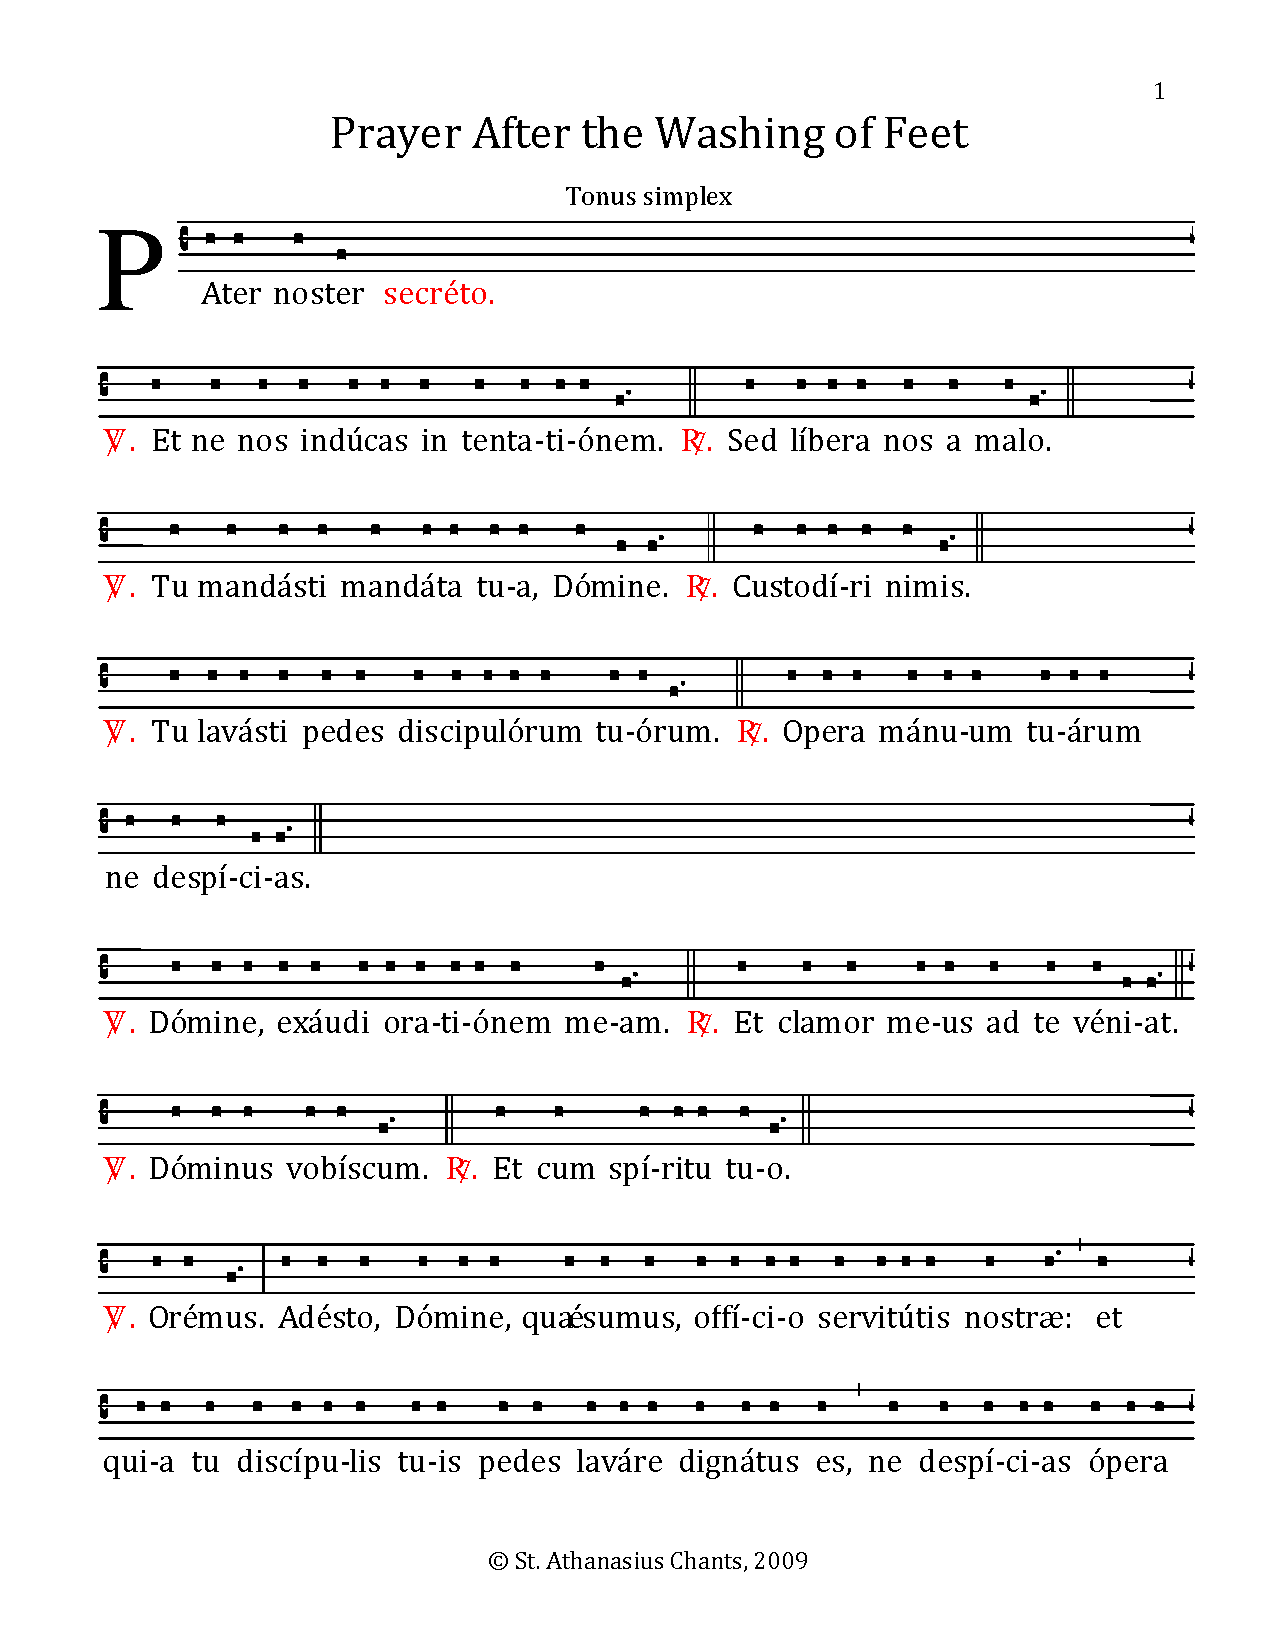
\includepdf[pages=-,pagecommand={},width=\textwidth]{Figures/Palmowa/prayer.pdf}



